\documentclass{sysuthesis}



%题目
\title{基于压缩文本的字符串近似查询算法研究}
%作者
\author{李贝瑀}
%院系
\school{数据科学与计算机学院}
%专业
\major{计算机科学与技术}
%学生
\student{李贝瑀}
%学号
\studentid{11318030}
%指导教师
\mentor{林瀚(讲师)}
%日期
\date{二〇一六年四月}



%开题报告正文
\openingrep{
	选题目的\\
	如何高效的存储大量字符串以及快速检索其中相近的子集,在基因组序列、Wiki条目等问题中起着关键的作用。目前较多的方法只侧重于其中一点,即牺牲查找速度实现压缩存储,或建立大规模的索引加快搜索。因此,找出一种兼备存储效率及检索速度的方法很有实用意义。\\
	\\
	思路及方法\\
	对于文本压缩,比较常见的方法是对于某些近似的字符串,选出一个字符串作为它们的参考。该方法的问题在于,对于需要检索的字符串,只能找出与其近似的参考,而不是近似的字符串子集。
	在这个方法的基础上加以改进,我们可以构建分层结构的多重参考,即每个字符串存在多个参考,参考间存在层次化的依赖关系。对于检索,需要先找到匹配的参考,通过对参考中预处理信息的考察,得出所有与询问串编辑距离小于k的字符串集合。
	问题的难点在于,找出合适的算法与数据结构,用于构造字符串间的参考关系,在保证较高压缩率的同时,兼顾检索的速度。\\
	\\
	进度安排\\
	2015年12月 查看文献,总结他人在该类问题上的思路与技巧\\
	2016年03月 尝试多种算法及数据结构,测试比较并完成论文撰写\\
}

%开题报告指导教师意见
\openingopinion{
	海量数据的存储和检索是数据科学的重要问题,作者的选题有学术价值,也有技术难度。\\
}



%第一次过程检查的学生总结
\firstcheck{
	阅读了几篇关于字符串压缩、字符串k近似匹配的论文,学习了解决这两个问题较为常见的思路、方法。
}
%第一次过程检查的指导老师意见
\firstopinion{\rule{0cm}{2\baselineskip}}
%第二次过程检查的学生总结
\secondcheck{
	大致构建了压缩的算法、查询的算法框架,考虑用后缀数组或者后缀树做字符串匹配。\\
	从部分结果进行扩展时,似乎可以使用函数式线段树查询区间,但空间复杂度略高。
}
%第二次过程检查的指导老师意见
\secondopinion{\rule{0cm}{2\baselineskip}}
%第三次过程检查的学生总结
\thirdcheck{
	最终选择了较为简洁的后缀自动机作为主要的数据结构进行字符串匹配,区间的查询可用区间树维护。\\
	完成了总体的代码,压缩率一般,继续考虑较为细节的策略。
}
%第三次过程检查的指导老师意见
\thirdopinion{\rule{0cm}{2\baselineskip}}
%整体完成情况的指导老师意见
\overallopinion{\rule{0cm}{4\baselineskip}}



%指导教师评语
\instructorcomment{\rule{0cm}{6\baselineskip}}
%指导教师给予的成绩评定
\instructorgrade{\rule{0cm}{2\baselineskip}}
%答辩小组或专业负责人意见
\majorcomment{\rule{0cm}{4\baselineskip}}
%答辩小组或专业负责人给予的成绩评定
\majorgrade{\rule{0cm}{2\baselineskip}}
%院系负责人意见
\schoolcomment{\rule{0cm}{3\baselineskip}}
%院系负责人给予的成绩评定
\schoolgrade{\rule{0cm}{2\baselineskip}}



\cabstract{
	对于海量数据的存储与检索,是数据科学领域的重要问题,在构建人类基因库、Wiki文库历史版本维护等问题中起着关键作用。近年来,越来越多的研究开始将两者结合起来,在保证数据压缩存储的同时,兼备检索的能力。本文旨在利用一种较为简洁的数据结构——后缀自动机,对于可添加的字符串集合,动态构建包含多个引用的层次化索引结构,其中:1)引用的选择由程序自身决策,而非人工选择;2)支持基于编辑距离的近似字符串匹配。经证实,对于索引结构的字符串压缩方案来说,寻找空间最优解是一个NP-hard问题。因此,本文的最终目标在于尽量优化存储空间,在满足较高压缩率的同时,兼顾检索的速度。
}
\keywords{数据压缩;近似匹配;索引;后缀自动机}
\eabstract{
	Storing and searching of massive data is an important issue in the field of data science, which plays a key role in problems as construction of the human gene pool and in maintenance problems about historical versions in Wiki library. Recently, more and more researchers have been beginning to combine them. In other words, when it comes to the compressed storage of data, the searching ability is also demanded. This paper aims to use a relatively compact data structure - suffix automaton, to dynamically build the hierarchical index structure containing multiple reference, for the set of strings that can expand, in which: 1) the reference is selected by its own decision-making procedures, rather than artificial selection; 2) it is supported to match approximate string based on their edit-distance. It was confirmed that for the index structure string compression scheme, finding the optimal solution in space is an NP-hard problem. Therefore, the ultimate goal of this paper is trying to optimize storage space to meet the higher compression ratio while taking a efficent searching method into account.
}
\ekeywords{Compression; approximate matching; indexing; suffix automaton}



\begin{document}

\frontmatter

\cleardoublepage
\tableofcontents

\mainmatter



\chapter{引言}
在信息科学领域中,字符串及相关问题一直以来都是研究的热点,其中最具代表性的当属匹配[19]与压缩[]问题。在数据量越来越大的今天,直接对字符串本身进行存储将占用大量空间,如何在其中检索有用的信息也是一大难题。那么对于庞大的字符串集合,要如何将其压缩至尽量小的空间,却又可以尽量快的进行检索呢?



\section{背景}
近年来,随着信息技术在基因工程方面的普及,越来越多的DNA序列问题依赖计算机来处理。例如在研究基因突变时,由于突变率较低,必须记录下大量实验数据,再找出其中与原DNA序列近似的片段。其他方面,网络知识库的加速更迭,使得历史版本的存储带来挑战。在Wiki条目中,对于某个名词,可能存在许多类似的别称,需要一种近似检索的策略。\par
在字符串检索领域中有一种较为重要的方式——k近似匹配:在一个字符串集合中,找出与模式串之间编辑距离不超过k的所有子串,其中编辑距离表示将模式串通过插入、修改、删除变为目标串的最小修改次数。传统的k近似匹配基本只用到两种方法:1)对于集合内的字符串分别处理;2)将集合内的字符串拼接起来处理。这两种方法的局限性在于,存储所占用的空间至少是所有字符串长度之和。由于自然语言的特性,许多语句之间具有极强的关联性,可以通过其中的某一句话的片段,表达其他句子的部分信息,从而达到压缩存储的目的。因此,越来越多研究开始尝试先选择一些字符串作为索引,再将与之相似的串通过引用进行压缩的方法。此时,k近似匹配变成了两个问题:1)在索引集合中检索;2)找出与该索引串相似的引用串。这种方法的问题在于,只有索引中的匹配是精确的,引用串只是与索引串相似,而非模式串。\par
因此,找出一种将两者结合起来,在保证数据压缩存储的同时,兼备高效检索能力的算法是十分有意义的。



\section{相关成果}
我们首先简单介绍一下前人有关字符串压缩算法的研究成果,以及这一技术在解决各领域有关检索问题时的应用。



\subsection{字符串压缩}
字符串压缩是计算机科学及相关领域的经典问题。一种与本文相关的压缩方式,称为基于引用的压缩算法[21, 30],是将被压缩串替换为由其他串的片段构成的引用序列。压缩率取决于字符串间的相似程度,相似度越高则压缩的效果越好。对于某些基因片段来说,这一比率甚至可以达到1,000:1[36]。



\subsection{半结构化文档压缩}
对于倒排文档[4]的压缩一般应用于文本文档的储存中,主要思路是将所有出现的词组用标准压缩方式进行压缩,再基于词组进行索引。该方法对于大多数资料有较高的压缩效率[16],但并不支持字符串的近似检索。



\subsection{基于特殊领域的索引压缩}
对于字符串集合的管理在生物学中十分重要。最近,越来越多的算法致力于用树形的引用结构压缩基因组,并提供近似搜索的可能。该方法可以达到极高的压缩率,但对于大量的长字符串,压缩速度较低。其次,由于检索基于筛选出的特定序列,因此会遗漏部分结果。



\section{本文工作}
本文结合了前人的研究结果,尝试构建动态的多引用可搜索索引模型,支持动态扩展的字符串集合,通过多引用提高压缩率,自动决策引用的选择以及提供高效的搜索策略。构建思路的难点在于:1)每次要在原有结构的基础上进行简单修改即可完成更新,需要适合的数据结构;2)每个引用串可以引用多个不同的索引,需要在字符串集合中进行快速匹配,并设计尽量优化空间的选择策略;3)需要快速的k近似匹配算法,以及合适的数据结构维护引用的关系,从而递推出全部结果;4)特殊情况的处理。\par
下面我们将对上述问题依次讨论。



\chapter{压缩与索引}
这里我们介绍多引用索引结构的具体细节,随后我们建立简单的只通过主引用索引的结构,在此基础上再构建基于DAG(Directed Acyclic Graphs)的层次化引用。



\section{符号定义}
首先我们介绍一下本章节用到的定义及符号表示。\par
一个字符串$s$表示一个关于字符集$\Sigma$的有限序列,长度用$|s|$表示。两个字符串的连接用$s \circ t$表示。从下标$i$开始的长度为$n$的字符串用$s(i, n)$表示,特别的对于长度为$1$的子串(即一个字符)用$s(i)$表示,注意这里的下标从0开始。对于两个字符串$s$与$t$,如果他们之间的编辑距离不超过k,即$s$可以通过至多k次插入、修改、删除操作变为$t$,则称之$s$与$t$为k近似,记作$s \sim_{k} t$。\par
对于一个索引,我们用$RME$(Referential Match Entry)来表示,是由$(refid, start, length, mismatch)$组成的元组,其中$refid$是被引用串id,$start$表示起始位置,$length$表示长度,$mismatch$表示失配处的字符,即表示字符串$s_{refid}(start, length) \circ mismatch$。\par
对于一个压缩字符串,我们用$RCS$(Referential Compression Sequence)来表示,同时记录下其中每个$RME$的前缀长度$offset_{i}$。



\section{索引结构}
通常来说,在索引结构的字符串集合中,有一部分字符串是不经压缩直接保存的,称为主引用集合($PREF$)。除此之外,其他字符串都直接或间接使用主引用的子串作为索引,称为压缩集合($COMP$)。\par
需要注意的几点是,这里的主引用集合中可以存在多个字符串。这样的好处在于,由于主引用集合中的子串被引用的概率较高,可以提高压缩率。在储存时,只有主引用直接保存原文,其他字符串只保存$RCS$形式的索引信息。由于主引用集合一般较小,故大部分字符串还是以索引的形式保存的。为了方便实现,一般将主引用集合中的字符串也加入压缩集合中。其次,不是只有主引用才可以作为索引,每个串都可以被引用。这样可以防止主引用集合过于庞大,因为主引用集合是未经压缩的。但必须保证的是,互相之间的引用关系不会形成环。\par
下面,我们来看一个简单索引结构的构建。



\section{简单索引}
在最简单的版本中,每个串都只以主引用作为索引。\par
这里有一个样例,若字符串集合$S = \{s_{1}, s_{2}, ... s_{6}\}$,其中:\par
\hspace{1cm}$s_{1}$ = Aho–Corasick Automaton, $s_{2}$ = Aho/Corasick,\par
\hspace{1cm}$s_{3}$ = Aho/Corasick Automaton, $s_{4}$ = Aho/Corasick Automata,\par
\hspace{1cm}$s_{5}$ = Link-cut Tree, $s_{6}$ = LinkCut Tree.\par
对于$s_{2}$来说,引用$s_{1}$构成的$RCS$序列为$[(1, 0, 3, /), (1, 4, 7, k)]$,因为$s_{2} = s_{1}(0, 3) \circ / \circ s_{1}(4, 7) \circ k$。但对于$s_{5}$来说,这样显然就不合适了。因此,我们选择$s_{1}$与$s_{5}$作为主引用,即$PREF = \{s_{1}, s_{5}\}$。此时我们得到:\par
\hspace{1cm}$comp(s_{1}, \{s_{1}\}) = [(1, 0, 21, n)]$\par
\hspace{1cm}$comp(s_{2}, \{s_{1}\}) = [(1, 0, 3, /), (1, 4, 7, k)]$\par
\hspace{1cm}$comp(s_{3}, \{s_{1}\}) = [(1, 0, 3, /), (1, 4, 17, n)]$\par
\hspace{1cm}$comp(s_{4}, \{s_{1}\}) = [(1, 0, 3, /), (1, 4, 16, a)]$\par
\hspace{1cm}$comp(s_{5}, \{s_{5}\}) = [(5, 0, 12, e)]$\par
\hspace{1cm}$comp(s_{6}, \{s_{5}\}) = [(5, 0, 4, C), (5, 6, 6, e)]$\par
他们之间的引用关系如图\ref{imag_csimple}所示。\par

\begin{figure}[htbp]
\centering
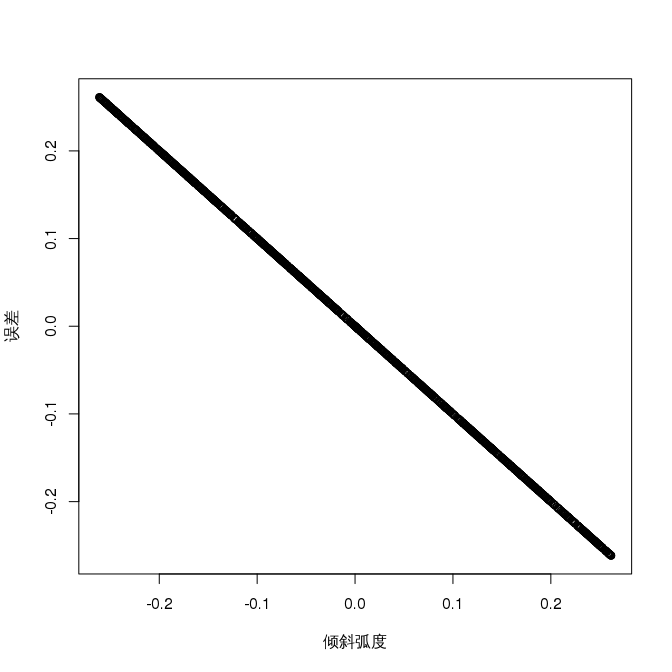
\includegraphics[scale=0.3]{image/err_ref.png}
\caption{简单索引}\label{imag_csimple}
\end{figure}

下面,我们来介绍构建的具体算法。\par
在初始状态下,有$PREF = \emptyset$,$COMP = \emptyset$。随后加入$s_{1}$时,由于$PREF$为空,$s_{1}$无法选择任何引用,故将$s_{1}$加入$PREF$,得到$PREF = \{s_{1}\}$,$COMP = \{s_{1}\}$。在加入$s_{2}$时我们有两种选择:1)将$s_{2}$加入$PREF$;2)以$s_{1}$作为引用构建索引。显然,当$s_{1}$与$s_{2}$较为相似时,选择后者较优,这时我们得到$PREF = \{s_{1}\}$,$COMP = \{s_{1}, s_{2}\}$。否则选择前者,此时$PREF = \{s_{1}, s_{2}\}$,$COMP = \{s_{1}, s_{2}\}$。加入$s_{3}$时,要先与$PREF$中的所有主引用比较相似度,再进行决策。\par
然而相似度的概念过于主观,因此我们的算法需要一定的策略来选择加入的方式,流程如算法\ref{algo_csimple}所示。\par

\begin{algorithm}[H]
	\SetKwData{PREF}{PREF}\SetKwData{COMP}{COMP}\SetKwData{rcs}{rcs}\SetKwData{cost}{cost}
	\SetKwFunction{Comp}{comp}\SetKwFunction{Sizeof}{sizeof}
	\SetKwInOut{Input}{input}\SetKwInOut{Output}{output}
	\Input{String sequence $S = \{s_{1}, s_{2}, ... , s_{n}\}$}
	\Output{Simple Compression}
	\PREF $\leftarrow \emptyset$\;
	\COMP $\leftarrow \emptyset$\;
	\For{$i \leftarrow 1$ \KwTo $n$}{
		\cost $\leftarrow \infty$\;
		\If{$|$\PREF$|$ $>$ 0}{
			\rcs $\leftarrow$ \Comp{$s_{i}$, \PREF}\;
			\cost $\leftarrow$ \Sizeof{\rcs}\;
		}
		\If{\cost $<$ \Sizeof{$s_{i}$}}{
			\COMP $\leftarrow$ \COMP $\cup$ \{\rcs\}\;
		}
		\Else{
			\PREF $\leftarrow$ \PREF $\cup$ \{\rcs\}\;
			\COMP $\leftarrow$ \COMP $\cup$ \{$(s_{i}, 0, |s_{i}| - 1, s_{i}(|s_{i}| - 1))$\}\;
		}
	}
	\caption{Computation of Simple Compression}\label{algo_csimple}
\end{algorithm}



\chapter{模版使用说明}

\section{正常使用}

本模版主要组成部分有:

\begin{itemize}
\item {\ttfamily main.tex}为主文件,毕业论文的内容应放在这个文件中。
\item {\ttfamily main.bib}为参考文献记录。
\item {\ttfamily sysuthesis.bst}为参考文献样式文件。
\item {\ttfamily sysuthesis.cls}为文类文件,应与主文件放在相同的目录中。
\item {\ttfamily image/logo.png}为用在封面的校徽。
\end{itemize}

主文件{\ttfamily main.tex}基本上是自解释的。在正常使用时,只用按照源文件中注释在正确位置填写各种基本信息、开题报告内容和中英文摘要内容,然后把注释``现在开始正文''到注释``篇末注''之间部分替换为正文,再按照注释在正确位置加入参考文献、致谢和附录等。最后用{\ttfamily xelatex}编译即可:

\begin{lstlisting}[language=bash, keywordstyle=\color{blue}\bfseries, basicstyle=\ttfamily, breaklines=true, frame=shadowbox]
xelatex main
bibtex main
xelatex main
xelatex main
\end{lstlisting}
。当然也可以用{\ttfamily makefile}或用脚本简化编译过程。

\section{配置}

在使用本模版前,请先保证已安装以下宏包:

\begin{itemize}
\item {\ttfamily ctex}
\item {\ttfamily tocloft}
\item {\ttfamily calc}
\item {\ttfamily graphicx}
\item {\ttfamily amsmath}
\item {\ttfamily amssymb}
\item {\ttfamily amsthm}
\item {\ttfamily listings}
\item {\ttfamily subfig}
\item {\ttfamily longtable}
\item {\ttfamily endnotes}
\item {\ttfamily algorithm2e}
\item {\ttfamily hyperref}
\item {\ttfamily placeins}
\end{itemize}

为了让{\ttfamily algorithm2e}宏包支持中文,请把该宏包的文件{\ttfamily algorithm2e.sty}(在我的系统中,它在{\ttfamily /usr/share/texlive/texmf-dist/tex/latex/algorithm2e/})替换为本模版附带的同名文件。不需要描述算法时,可以在{\ttfamily sysuthesis.cls}中去掉以下代码
\begin{lstlisting}[language=TeX, keywordstyle=\color{blue}\bfseries, basicstyle=\ttfamily, breaklines=true, frame=shadowbox]
\RequirePackage[chinese,onelanguage,noline,noend,linesnumbered]{algorithm2e}
\end{lstlisting}
并在主文件中去掉以下代码
\begin{lstlisting}[language=TeX, keywordstyle=\color{blue}\bfseries, basicstyle=\ttfamily, breaklines=true, frame=shadowbox]
\listofalgorithms
\end{lstlisting}
(源文件有注释提示)。

如果在windows编译且希望使用微软的字体时,请把{\ttfamily sysuthesis.cls}中以下代码
\begin{lstlisting}[language=TeX, keywordstyle=\color{blue}\bfseries, basicstyle=\ttfamily, breaklines=true, frame=shadowbox]
\LoadClass[adobefonts,a4paper,openright,cs4size,fancyhdr]{ctexbook}[2010/01/22]
\end{lstlisting}
改为
\begin{lstlisting}[language=TeX, keywordstyle=\color{blue}\bfseries, basicstyle=\ttfamily, breaklines=true, frame=shadowbox]
\LoadClass[winfonts,a4paper,openright,cs4size,fancyhdr]{ctexbook}[2010/01/22]
\end{lstlisting}。

如果想使用开源字体{\ttfamily Fandol}(假定已安装它),请把{\ttfamily ctex}宏包的文件{\ttfamily ctex-xecjk-adobefonts.def}(在我的系统中,它在{\ttfamily /usr/share/ texlive/texmf-dist/tex/latex/ctex/fontset/})替换为本模版附带的同名文件。

关于参考文献的bib条目格式参考\texttt{main.bib}~\cite{article}\cite{book}\cite{phdthesis}\cite{inproc}\cite{masterthesis}\cite{manual}\cite{report}\cite{database}\cite{software}\cite{standard}\cite{newspaper}\cite{patent}。

\chapter{写作时的注意事项}

本章列出一些本模板未能规范也不太适合以注释形形式写在源文件的要求,请使用者注意。

\section{毕业论文的撰写内容与要求}

正文一般包括以下几个方面:

\begin{enumerate}
\item 引言或背景\\
引言是论文正文的开端,应包括毕业论文选题的背景、目的和意义;对国内外研究现状和相关领域中已有的研究成果的简要评述;介绍本项研究工作研究设想、研究方法或实验设计、理论依据或实验基础;涉及范围和预期结果等。要求言简意赅,注意不要与摘要雷同或成为摘要的注解。
\item 主体\\
论文主体是毕业论文的主要部分,必须言之成理,论据可靠,严格遵循本学科国际通行的学术规范。在写作上要注意结构合理、层次分明、重点突出,章节标题、公式图表符号必须规范统一。论文主体的内容根据不同学科有不同的特点,一般应包括以下几个方面:
\begin{itemize}
\item 毕业论文(设计)总体方案或选题的论证;
\item 毕业论文(设计)各部分的设计实现,包括实验数据的获取、数据可行性及有效性的处理与分析、各部分的设计计算等;
\item 对研究内容及成果的客观阐述,包括理论依据、创新见解、创造性成果及其改进与实际应用价值等;
\item 论文主体的所有数据必须真实可靠,凡引用他人观点、方案、资料、数据等,无论曾否发表,无论是纸质或电子版,均应详加注释。自然科学论文应推理正确、结论清晰;人文和社会学科的论文应把握论点正确、论证充分、论据可靠,恰当运用系统分析和比较研究的方法进行模型或方案设计,注重实证研究和案例分析,根据分析结果提出建议和改进措施等。
\end{itemize}
\item 结论\\
结论是毕业论文的总结,是整篇论文的归宿,应精炼、准确、完整。结论应着重阐述自己的创造性成果及其在本研究领域中的意义、作用,还可进一步提出需要讨论的问题和建议。
\end{enumerate}

\section{毕业论文的撰写格式要求}

除有特殊要求的专业外,毕业论文正文一般不少于 5000 字。各专业可根据需要确定具体的文字和字数要求,并报教务处备案。

正文各部分的标题应简明扼要,不使用标点符号。

名词术语的要求:

\begin{itemize}
\item 科学技术名词术语尽量采用全国自然科学名词审定委员会公布的规范词或国家标准、部标准中规定的名称,尚未统一规定或叫法有争议的名词术语,可采用惯用的名称。
\item 特定含义的名词术语或新名词、以及使用外文缩写代替某一名词术语时 , 首 次 出 现 时 应 在 括 号 内 注 明 其 含 义 , 如 : OECD ( Organisation for Economic Co-operation and Development) 代替经济合作发展组织。
\item 外国人名一般采用英文原名,可不译成中文,英文人名按姓前名后的原则书写,如:CRAY P,不可将外国人姓名中的名部分漏写,例如:不能只写CRAY, 应写成 CRAY P。一般很熟知的外国人名(如牛顿、爱因斯坦、达尔文、马克思等)可按通常标准译法写译名。
\end{itemize}

物理量名称、符号与计量单位的要求:

\begin{itemize}
\item 论文中某一物理量的名称和符号应统一,一律采用国务院发布的《中华人民共和国法定计量单位》。单位名称和符号的书写方式,应采用国际通用符号。
\item 在不涉及具体数据表达时允许使用中文计量单位如“千克”。
\item 表 达 时 刻 应 采 用 中 文 计 量 单 位 , 如 “ 下 午 3 点 10 分 ” , 不 能 写 成“3h10min”,在表格中可以用“3:10PM”表示。
\item 物理量符号、物理量常量、变量符号用斜体,计量单位符号均用正体。
\end{itemize}

数字的要求:

\begin{itemize}
\item 无特别约定情况下,一般均采用印度——阿拉伯数字表示。
\item 年份一律使用 4 位数字表示。
\item 小数的表示方法:一般情形下,小于 1 的数,需在小数点之前加 0。但当某些特殊数字不可能大于 1 时(如相关系数、比率、概率值),小数点之前的 0 要去掉,如 r=.26,p<.05。
\item 统计符号的格式:一般除 μ、α、β、λ、ε 以及 V 等符号外,其余统计符号一律以斜体字呈现,如ANCOVA , ANOVA , MANOVA , N , nl , M , SD , F , p , r 等。
\end{itemize}

公式的要求:

\begin{itemize}
\item 公式应另起一行写在稿纸中央。一行写不完的长公式,最好在等号处转行,如做不到这一点,可在运算符号(如“+”、“-”号)处转行,等号或运算符号应在转行后的行首。
\item 公式的编号用圆括号括起,放在公式右边行末,在公式和编号之间不加虚线。公式可按全文统编序号,也可按章独立序号,如(49)或(4.11)。采用哪一种序号应和图序、表序编法一致。不应出现某章里的公式编序号,有的则不编序号。子公式可不编序号,需要引用时可加编 a、b、c......,重复引用的公式不得另编新序号。公式序号必须连续,不得重复或跳缺。
\item 文中引用某一公式时,写成“由式(16.20)”。
\end{itemize}

表格的要求(表\ref{tab:skew}为一个也许不合格的例子):

\begin{itemize}
\item 表格必须与论文叙述有直接联系,不得出现与论文叙述脱节的表格。表格中的内容在技术上不得与正文矛盾。
\item 每个表格都应有自己的标题和序号。标题应写在表格上方正中,不加标点,序号写在标题左方。
\item 全文的表格可以统一编序,也可以逐章单独编序。采用哪一种方式应和插图、公式的编序方式统一。表序必须连续,不得跳缺。
\item 表格允许下页接写,接写时标题省略,表头应重复书写,并在右上方写“续表××”。多项大表可以分割成块,多页书写,接口处必须注明“接下页”、“接上页”、“接第×页”字样。
\item 表格应放在离正文首次出现处最近的地方,不应超前和过分拖后。
\end{itemize}

\begin{table}[hbp]
\caption{各个倾斜校正方法性能对比}
\centering
\begin{tabular}{lrrrrr}
\hline
& 成功返回率 & 平均误差& 均方误差& 误差中位数& 运行时间中位数\\
& & (弧度) & (弧度) & (弧度) & (毫秒)\\\hline
参照方法&$\mathbf{100.00\%}$&0.1298&0.1504&0.1286&$\mathbf{0}$\\
分片填涂方法&93.48\%&0.0621&0.1947&0.0061&50\\
分片覆盖方法&99.10\%&0.0154&$\mathbf{0.0299}$&0.0073&300\\
投影方法&99.35\%&$\mathbf{0.0068}$&0.0335&$\mathbf{0.0033}$&197\\
交错数方法&99.35\%&0.0101&0.0458&0.0035&198\\
霍夫变换方法&99.35\%&0.1448&0.1827&0.0452&99\\
行间相关方法&93.81\%&0.2115&0.3811&0.0346&1615\\
最近邻方法&96.71\%&0.0883&0.1207&0.0690&67\\\hline
\end{tabular}
\label{tab:skew}
\end{table}

图的要求(图\ref{fig:skew}为一个也许不合格的例子):

\begin{itemize}
\item 插图应与文字内容相符,技术内容正确。所有制图应符合国家标准和专业标准。对无规定符号的图形应采用该行业的常用画法。
\item 每幅插图应有标题和序号,全文的插图可以统一编序,也可以逐章单独编序,如:图 45 或图 6.8。采取哪一种方式应和表格、公式的编序方式统一。图序必须连续,不重复,不跳缺。
\item 由若干分图组成的插图,分图用 a、b、c......标序。分图的图名以及图中各种代号的意义,以图注形式写在图题下方,先写分图名,另起行写代号的意义。
\item 图与图标题、图序号为一个整体,不得拆开排版为两页。当页空白不够排版该图整体时,可将其后文字部分提前,将图移至次页最前面。
\item 对坐标轴必须进行文字标示,有数字标注的坐标图必须注明坐标单位。
\end{itemize}

\begin{figure}[htbp]
\centering
\subfloat[参照方法]{
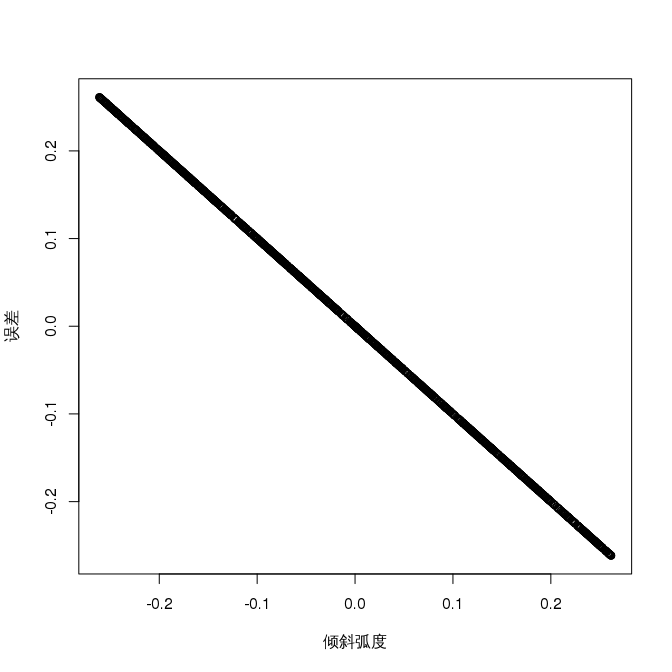
\includegraphics[scale=0.15]{image/err_ref.png}
}
\subfloat[分片填涂方法]{
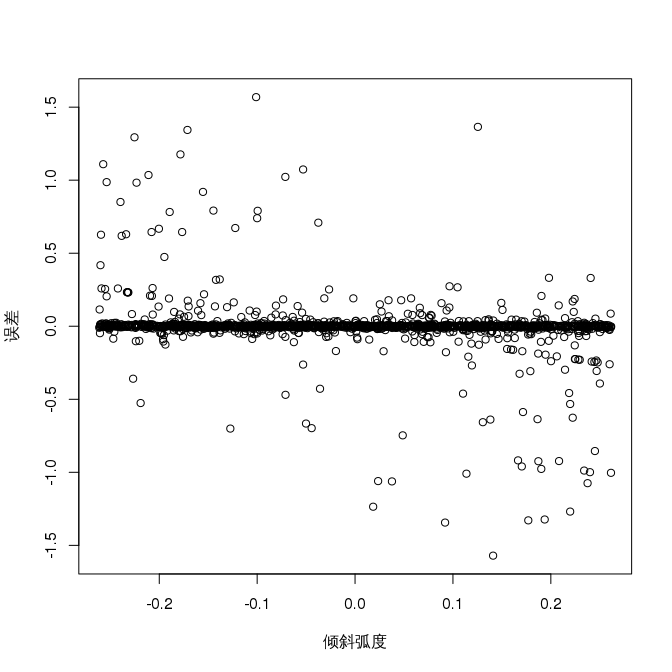
\includegraphics[scale=0.15]{image/err_ppa.png}
}\\
\subfloat[分片覆盖方法]{
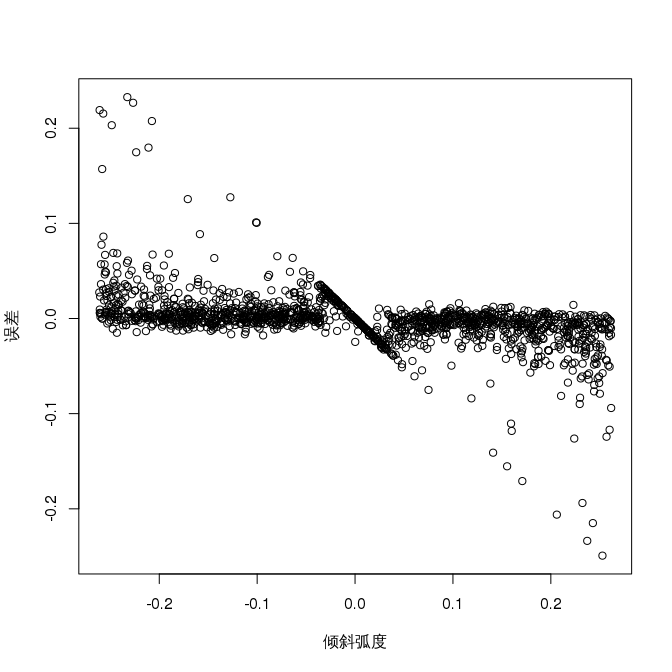
\includegraphics[scale=0.15]{image/err_pcp.png}
}
\subfloat[投影方法]{
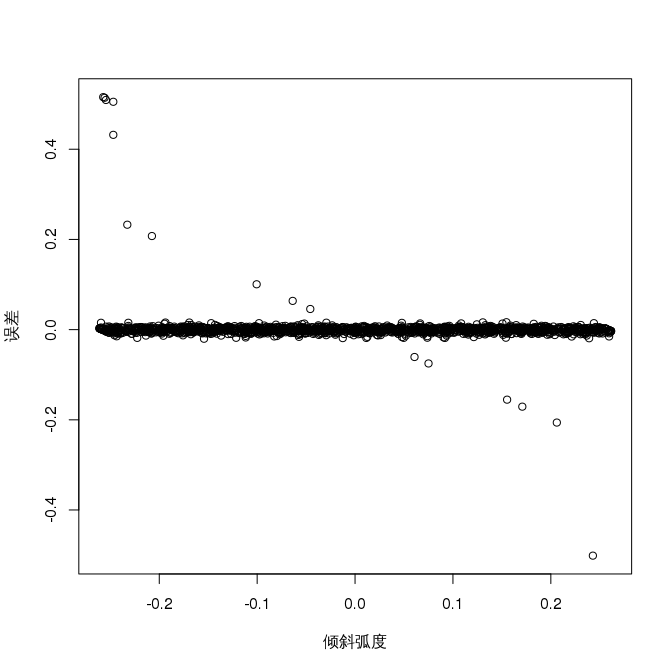
\includegraphics[scale=0.15]{image/err_pp.png}
}\\
\subfloat[交错数方法]{
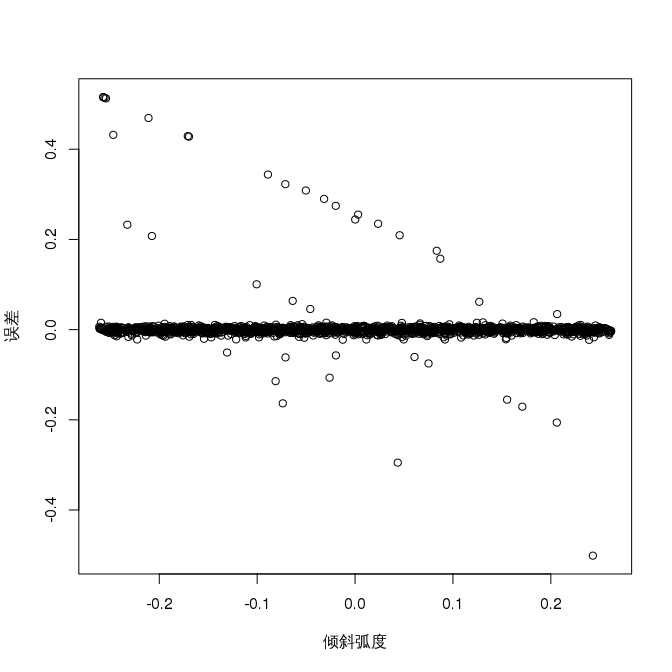
\includegraphics[scale=0.15]{image/err_tc.png}
}
\subfloat[霍夫变换方法]{
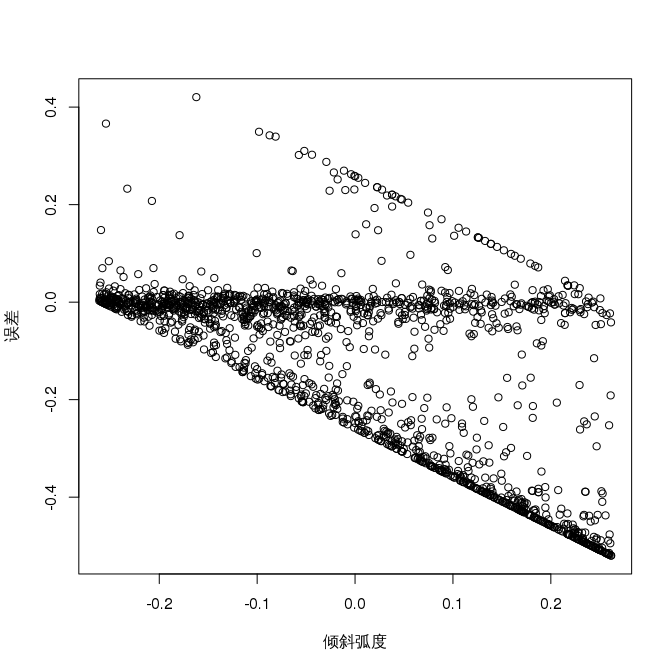
\includegraphics[scale=0.15]{image/err_ht.png}
}\\
\subfloat[行间相关方法]{
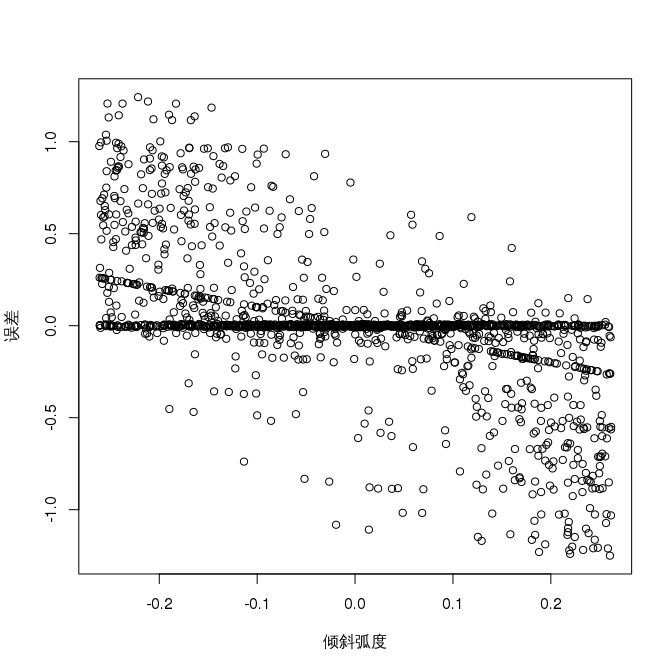
\includegraphics[scale=0.15]{image/err_cc.png}
}
\subfloat[最近邻方法]{
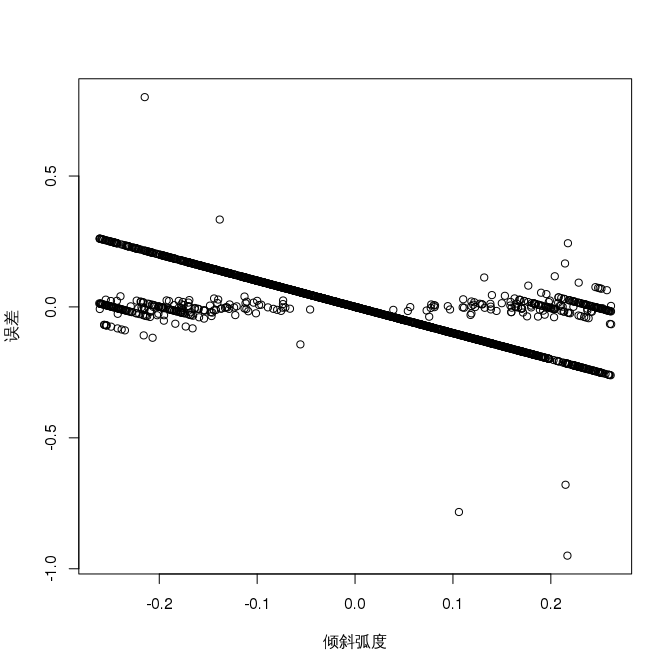
\includegraphics[scale=0.15]{image/err_nn.png}
}
\caption{各个倾斜校正方法的残差图}
\label{fig:skew}
\end{figure}

\chapter{结论}

\section{取得成果}

一个大概不为人知的模版,可以认为对于人类无任何贡献。

\section{后续工作}

此模版有以下已知局限性:

\begin{itemize}
\item 篇末注只支持最多10个
\item 有时用户可能要直接修改cls文件
\item 遗留了一些格式化代码在tex文件
\end{itemize}


%篇末注(非常抱歉只支持最多10个,在正文通过\endnote{}命令生成)
%\displayendnotes

%参考文献是毕业设计(论文)不可缺少的组成部分,它反映毕业设计(论文)的取材来源、材料的广博程度和材料的可靠程度,也是作者对他人知识成果的承认和尊重。一份完整的参考文献可向读者提供一份有价值的信息资料,列入的文献应在 10 篇以上,其中外文文献在 2 篇以上。
\zihao{-5}\songti
\bibliographystyle{sysuthesis}
\bibliography{main}%假定bib文件为main.bib

\appendix

\begin{thankto}

\songti\zihao{-4}
%谢辞应以简短的文字对课题研究与论文撰写过程中曾直接给予帮助的人员(例如指导教师、答疑教师及其他人员)表示对自己的谢意,这不仅是一种礼貌,也是对他人劳动的尊重,是治学者应当遵循的学术规范。内容限一页。
%以下为致谢内容
致谢内容

\vskip 18pt
\begin{flushright}
作者\\
\today
\end{flushright}
\end{thankto}

%对于一些不宜放在正文中的重要支撑材料,可编入毕业论文的附录中。包括某些重要的原始数据、详细数学推导、程序全文及其说明、复杂的图表、设计图纸等一系列需要补充提供的说明材料。如果毕业设计(论文)中引用的实例、数据资料,实验结果等符号较多时,为了节约篇幅,便于读者查阅,可以编写一个符号说明,注明符号代表的意义。附录的篇幅不宜太多,一般不超过正文。
%接下来是附录部分,以\chapter{附录标题}开始一个新的附录
\chapter{记号约定}
\songti\zihao{-4}
\begin{longtable}{ll}
记号 & 说明\\
\endfirsthead
记号 & 说明\\
\endhead
\endfoot
\endlastfoot
$A \cup B$ & 集合$A$与集合$B$的并集\\
$A \cap B$ & 集合$A$与集合$B$的交集\\
$A \setminus B$ & 集合$A$与集合$B$的差集\\
$A \times B$ & 集合$A$与集合$B$的直积\\
$A / \simeq$ & 集合$A$关于等价关系$\simeq$的商集\\
\end{longtable}

\backmatter

\end{document}
